%!TEX root = ../schoedon.tex

%%%%%%%%%%%%%%%%%%%%%%%%%%%%%%%%%%%%%%%%%%%%%%%%%%%%%%%%%%%%%%%%%%%%%%%%%%%%%%%%
\cleardoublepage              %%% IMPLEMENTATION                             %%%
\chapter{Web-based proof-of-concept}
  \label{chap:imple}
  A proof-of-concept implementation is provided along with this thesis. This
  chapter covers the Leaflet-JS integration details. It is targeted to work with
  web applications and mobile devices. In the following subsections the
  challenges with the web-based provision are examined. The architecture will be
  explained and the resulting applications will be presented.\par

  \section{Architecture overview}
    \label{sec:imple:archi}
    The implementation requires a client/server architecture which offers both,
    a tiling service supplying the pre-calculated glTF tiles and a routing
    service supplying travel times on-request at runtime (figure
    \ref{fig:imple:archi}).\par

    \begin{figure}[h]
      \centering
      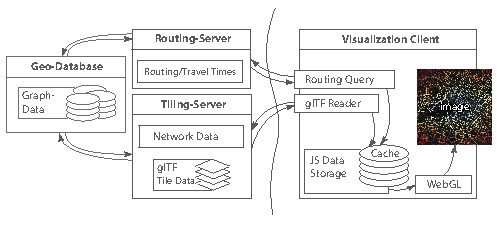
\includegraphics[width=\linewidth]{./img/conceptual-overview-bw.pdf}
      \caption{Architecture of preprocessing back-end and visualization client.}
      \label{fig:imple:archi}
    \end{figure}

    The back-end consists of three components:\par

    \begin{description}
      \item[Geo-Database] A geographic database server contains the street and
        transportation networks. It maintains updates from a remote geo-data
        source, e.g., OpenStreetMap, and processes the data into a
        routing-enabled graph representation.
      \item[Tiling-Server] A tiling server processes the static network data
        into a tiled glTF data set. This data only has to be generated once and
        will be available on-demand for any future geometry requests.
      \item[Routing-Server] A routing server handles dynamic requests based on
        the user's selected starting location, transportation type and maximum
        travel time. It responds with customized routing information for the
        underlying transportation network.
    \end{description}

    The front-end contains the mapping and rendering stages. A glTF reader will
    request and load the network geometries. Based on the user inputs, routing
    data will be queried. All responses are mapped, cached and rendered in the
    client.\par

    As described in section \ref{sec:conct:preli:backe}, the back-end is not
    subject to further technical specification in this document. Therefore, the
    following applications strongly focus on the front-end implementation and
    visualization.\par

  \section{Iterative development process}
    \label{sec:imple:cycle}
    The implementation is solved by an evolutionary prototyping process.\par

    To allow a fast evaluation of the results gained during the different stages
    of development, an evolutionary development process is used. It leads to
    multiple proof-of-concept versions which can be analyzed afterwards.\par

    A working back-end -- as specified in section \ref{sec:conct:preli:backe} --
    provides the prototypes with real-time data at run-time. It is provided and
    maintained by Motion Intelligence GmbH. By utilizing and extending the
    existing Route360-JS API [??], compatibility and potential future
    integrations are maintained.\par

  \section{Proof-of-concept applications}
    \label{sec:imple:applc}
    In the following sections, three major proof-of-concept implementations will
    be presented:\par

    \begin{description}
      \item[PoC\#1 Leaflet-JS with CPU native lines vector
        tiling] This implementation is not interesting for
        this work as it neither uses WebGL nor glTF and is only implemented to
        have a classic approach available. In addition, the performance of the
        first prototype is very low, even for small accessibility map
        visualizations (below 10 minutes travel time complexity in a city
        center, compare section \ref{sec:imple:applc:nativ}).
      \item[PoC\#2 Leaflet-JS with GPU-enabled canvas overlay and vector tiling]
        This prototype is interesting both for the successful
        WebGL integration in Leaflet-JS and the issues arising with GeoJSON
        post-processing. See section \ref{sec:imple:applc:vectr} for more
        details.
      \item[PoC\#3 Leaflet-JS with GPU buffer tiling] This approach
        is implementing a GPU buffer tiling service explicitly utilizing the
        glTF data exchange format. See section \ref{sec:imple:applc:tgltf} for
        more details.
    \end{description}

    \subsection{Leaflet-JS native network rendering}
      \label{sec:imple:applc:nativ}
      A reference implementation in Leaflet-JS is provided (figure
      \ref{fig:imple:applc:nativ}). It does not utilize hardware acceleration or
      WebGL rendering. It processes the vector data in GeoJSON format using the
      native Leaflet-JS JavaScript class \texttt{L.GeoJson}. Therefore, both the
      mapping and rendering will be performed on CPU.\par

      \begin{figure}[h]
        \centering
        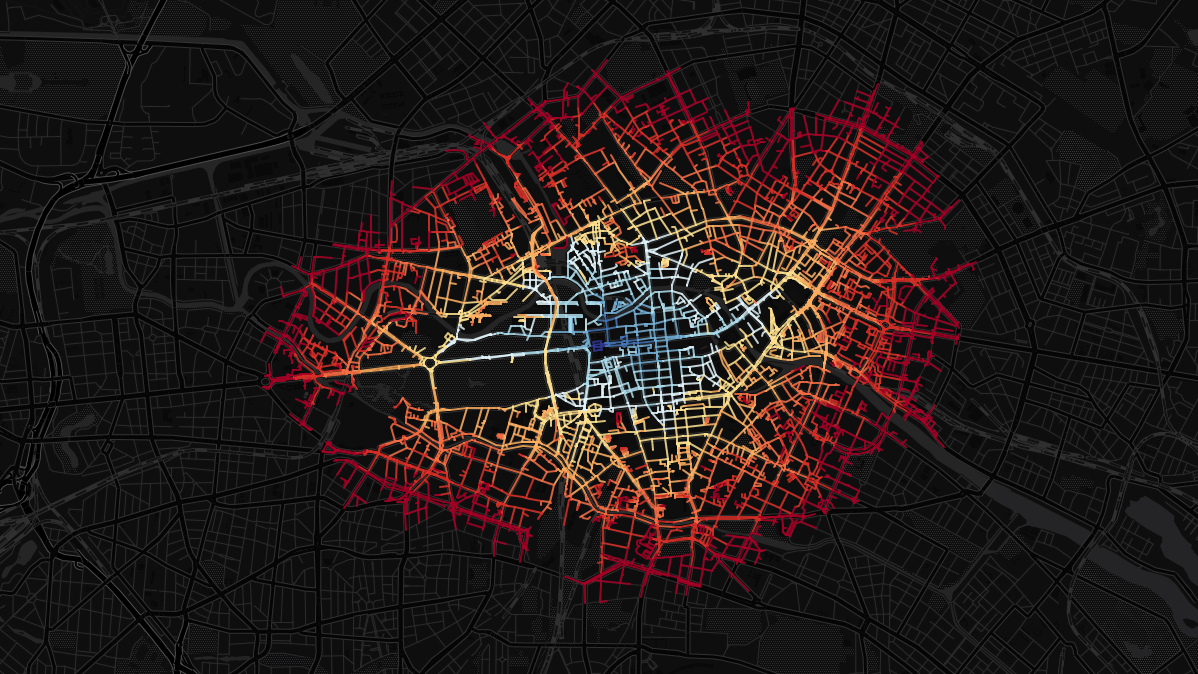
\includegraphics
          [width=0.7\linewidth]
          {./img/screenshot-poc1-600s-native.png}
        \caption{An accessibility map rendered native with Leaflet-JS vector
          tiles in GeoJSON format. The selected transportation mode is walking
          and the displayed travel time is 10 minutes.}
        \label{fig:imple:applc:nativ}
      \end{figure}

      The rendered street network for 600 seconds travel time in walking mode
      contains 13,829 features (25,821 vertices). It shows a major performance
      bottleneck for both the mapping and the rendering stage. It wont be
      evaluated any further and is only used for the performance comparison in
      section \ref{sec:evalu:pcomp} as native Leaflet-JS reference without
      WebGL hardware acceleration.\par

    \subsection{WebGL with tiled vector data}
      \label{sec:imple:applc:vectr}
      Leaflet-JS provides a 2D \texttt{L.map()} canvas on a
      \texttt{<div id="map" />} HTML DOM element. This can be used for basic web
      mapping tools like raster base tiles or simple vector items. The extended
      class \texttt{L.canvasOverlay()} by Sumbrera (2015) [??] provides
      Leaflet-JS with a 3D overlay which handles redrawing of the canvas and
      therefore allows basic WebGL context integration (figure
      \ref{fig:imple:applc:overlay}).\par

      % https://blog.sumbera.com/2014/04/20/leaflet-canvas/

      \begin{figure}[h]
        \centering
        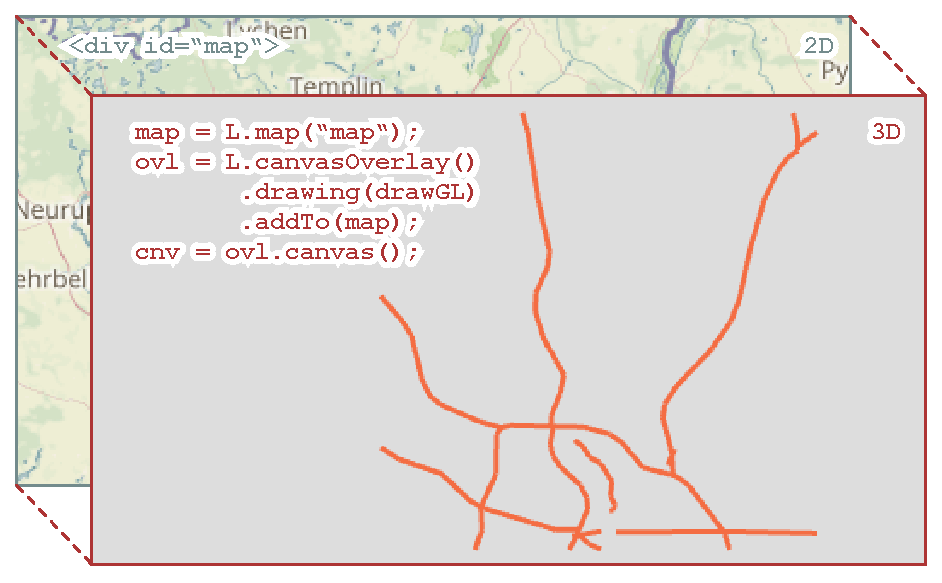
\includegraphics[width=0.7\linewidth]{./img/leaflet-canvas-overlay.pdf}
        \caption{Leaflet-JS canvas overlay schematic: A 2D map canvas is provided by Leaflet, the overlay class allows the rendering of 3D contexts.}
        \label{fig:imple:applc:overlay}
      \end{figure}

      On each map interaction, a \texttt{drawGL()} rendering call will be
      triggered by the overlay. This function reads the underlying GeoJSON and
      extracts all geographic features. For each feature in the feature-set, the
      algorithm checks the travel time properties and decides whether the
      feature is visible (below selected threshold) or not.\par

      Each visible feature will be converted to typed array buffers for vertices
      and colours. Each coordinate of the geometry has to be mapped to pixel
      coordinates (see section \ref{sec:conct:preli:gproj}).\par

      %%% @TODO below %%%

      The Leaflet-JS web-mapping framework does not offer any WebGL support, yet. Sumbrera [??] published a Leaflet-JS canvas overlay class which provides a generic overlay over the map canvas and handles view-port coordinates and drawing events.\par
      \lstinputlisting[float,caption={Leaflet-JS canvas overlay},label={lst:poc:overlay}]{./lst/leaflet-canvas-overlay.js}
      While Leaflet-JS provides a map canvas on a HTML DOM element (e.g., \texttt{<div id='map'>}) for two dimensional vector and raster contexts, Figure {fig:poc:overlay} shows how the \texttt{L.CanvasOverlay} class provides an additional context. The overlay can be used for custom HTML5 elements and handles view port coordinate alignment along with the underlying map. Furthermore, it can be utilized to bind a three dimensional context like WebGL and to handle the redrawing of the scene each time the map view changes (Listing {lst:poc:overlay}).\par
      \begin{figure}[h]
        \centering
        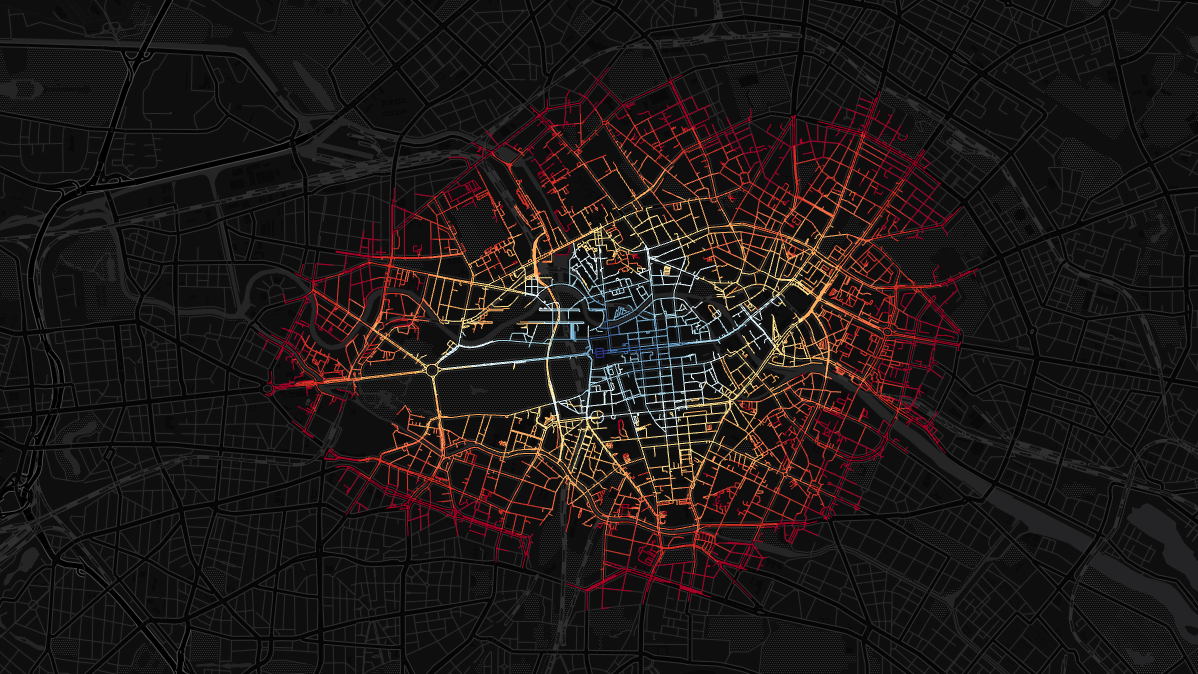
\includegraphics[width=0.7\linewidth]{./img/screenshot-poc2-600s-vector.png}
        \caption{An accessibility map rendered with WebGL on a Leaflet-JS canvas overlay utilizing vector tiles in GeoJSON format. The selected transportation mode is walking and the displayed travel time is 10 minutes.}
        \label{fig:poc:two}
      \end{figure}
      This implementation shows two issues.\par
      A blocking performance issue is the conversion from geodata to array buffers. For the mentioned dataset of only 15 minutes travel time this results in an iteration over 29.864 geographic features. In addition, the coordinates have to be iterated as well, leaving this example with 129.034 spheric conversions for 64.517 coordinates.\par
      Another problem is the unability to access the internal \texttt{EPSG :3857} metric coordinates from Leaflet. All positions have to be transformed using compute-intense spherical (degree) rather than optimized metric conversions [??].\par
      Leaflet-JS provides a 2D canvas on a HTML DOM element that is used for basic
      web-mapping tools such as raster-based tiles or simple vector items. An extended
      \textsl{canvas overlay} class provides Leaflet-JS with a 3D overlay that handles
      re-drawing of the canvas and enables basic WebGL context integration. On each map
      interaction, a draw call is issued by the overlay. This function processes the
      underlying GeoJSON and (1) extracts all geographic features, (2) marks each feature
      visible, if its travel time is below a user-selected threshold, and (3) converts
      each visible feature to typed array buffers (vertices and colors), including coordinate mapping.\par
      This implementation approach shows two performance bottlenecks: (1) the conversion
      from geodata representation to GPU array-buffers and (2) coordinate transformations
      for rendering~(cf.~Sec.~{WD:SubSec:PerformanceEvaluation}). \par
    \subsection{WebGL with tiled glTF data}
      \label{sec:imple:applc:tgltf}
      Table {tab:tilopts} highlights the advantages of geometry tiling. The layout stays dynamic and can be adjusted at runtime by custom user inputs similar to vector tiling approaches.\par
      The data processing is moved from client-side to server-side similar to raster tiling approaches. The result is high runtime preformance with low latencies and the resulting geometries can be cached client-side.\par
      The rendering happens on dedicated graphic devices and ensures outstanding performance even for complex geodata sets.

%%%      \begin{table}[!h]
%%%        \centering
%%%        \begin{tabular}{l|l|l|l}
%%%          Tile & Layout & Processing & Rendering\\ \hline
%%%          \cellcolor{yellow!15}Raster & \cellcolor{red!15}static & \cellcolor{green!15}Server & \cellcolor{red!15}Server\\
%%%          \cellcolor{yellow!15}Vector & \cellcolor{green!15}dynamic & \cellcolor{red!15}Client/CPU & \cellcolor{green!15}Client/GPU\\
%%%          \cellcolor{green!15}Geometry & \cellcolor{green!15}dynamic & \cellcolor{green!15}Server & \cellcolor{green!15}Client/GPU\\
%%%        \end{tabular}
%%%        \caption{Tiling options}
%%%        \label{tab:tilopts}
%%%      \end{table}
      Figure {fig:geotile} shows a screenshot of a modified version of the 4th prototype. It displays the geometry tile \texttt{[2200,1343]} at zoom level 12 rendered with WebGL using random colours.

%%%      \begin{figure}[h]
%%%        \centering
%%%        \includegraphics[width=0.475\textwidth]{resources/geometry-tile.png}
%%%        \caption{Geometry tile rendered with WebGL.}
%%%        \label{fig:geotile}
%%%      \end{figure}
      Two Leaflet-JS plugins are being developed to manage the tiling data logic [??].\par
      \begin{itemize}
        \item \texttt{L.TileBuffer} is the actual class for all geometry tiles. Each instance has the properties of \texttt{x}, \texttt{y} and \texttt{zoom}. In addition it stores the three required typed array buffers to render the tile with WebGL: a \texttt{Float32Array} for vertices, a \texttt{Uint16Array} for indices and a \texttt{Float32Array} for colours. This information is enough to render the complete tile in a single draw call.
        \item \texttt{L.TileBufferCollection} is a class which implements the basic tile caching logic. It has a \texttt{zoom} and a \texttt{size} property. In addition, it holds a collection of \texttt{L.Tile\-Buffer} objects for the current zoom level. As soon as the client requests a redraw of the scene, the collection can be rendered based on zoom and position of the visible tiles.
      \end{itemize}
      On each load event of a tile, Leaflet-JS will request the geometry (vertices and indices) from the tiling server and the travel times (colours) from the routing server. These three arrays are recieved in glTF format. They are used to create \texttt{L.TileBuffer} objects (figure {fig:tbuff}).\par

%%      \begin{figure}[h]
%%        \centering
%%        \includegraphics[width=0.3\textwidth]{resources/classes.pdf}
%%        \caption{Two Leaflet-JS plugins for geometry tiling.}
%%        \label{fig:tbuff}
%%      \end{figure}

      This approach eliminates client-side data processing and represents a new geometry-tiling
      approach based on glTF and following the common approach to partition map data
      into portions of similar size. Figure~{WD:Fig:ConceptualOverview} shows an conceptual
      overview of our approach: (1) the input transportation network will be pre-processed
      to glTF-tiles that are stored on a dedicated tiling server. In this step all
      coordinate transformations required for rendering are performed and a correspondence
      to the routing graph is established; (2) the visualization client queries the
      geometry of the tiles according to the current viewport and request travel times
      respectively by using the graph correspondence; (3) for visualization, the network
      tiles are cached and directly used for mapping and rendering.\par
      Table~{WD:Tab:TilingOptions} highlights the advantages of glTF-tiling. It
      supports client-side mapping (e.g., color mapping and lines styles) at runtime
      on according to user inputs without retransmission of data, similar to vector
      tiles. The data processing is transferred from client to server-side, similar
      to raster-tiling approaches. This results in high run-time performance with
      low latencies and the resulting geometries can be cached client-side. The
      rendering is performed on dedicated GPU using WebGL and thus ensures real-time
      performance for geometrical complex geodata sets.\par

      %%%%%%%%%%%%%%%%%%%%%%%%%%%%%%%%%%%%%%%%%%%%%%%%%%%%%%%%%%%%%%%%%%%%%%%%%%%%%%%
      %%
      %% Table: Tiling approaches
      %%
      %%%%%%%%%%%%%%%%%%%%%%%%%%%%%%%%%%%%%%%%%%%%%%%%%%%%%%%%%%%%%%%%%%%%%%%%%%%%%%%
%%      \begin{table}[b]
%%      \centering
%%      \beforeTable
%%      \begin{tabular}{|c|c|c|c|}
%%        \hline
%%        \textbf{Tiling Approach}  & \textbf{Processing}       & \textbf{Mapping}         & \textbf{Rendering}\\ \hline
%%        \cellcolor{yellow}Raster  & \cellcolor{green}Server   & \cellcolor{red}static    & \cellcolor{red}Server\\
%%        \cellcolor{yellow}Vector  & \cellcolor{red}Client/CPU & \cellcolor{green}dynamic & \cellcolor{green}Client/GPU\\
%%        \cellcolor{green}glTF     & \cellcolor{green}Server   & \cellcolor{green}dynamic & \cellcolor{green}Client/GPU\\
%%        \hline
%%      \end{tabular}
%%      \caption{Comparison and rating (dark background means not suitable) of tiling
%%      approaches with respect to the requirements of data processing, mapping, and
%%      rendering.}
%%      \label{WD:Tab:TilingOptions}
%%      \afterFloat
%%      \end{table}
      %%%%%%%%%%%%%%%%%%%%%%%%%%%%%%%%%%%%%%%%%%%%%%%%%%%%%%%%%%%%%%%%%%%%%%%%%%%%%%%

%%%%%%%%%%%%%%%%%%%%%%%%%%%%%%%%%%%%%%%%%%%%%%%%%%%%%%%%%%%%%%%%%%%%%%%%%%%%%%%%
